% This LaTeX was auto-generated from MATLAB code.
% To make changes, update the MATLAB code and republish this document.

\documentclass{article}
\usepackage{graphicx}
\usepackage{color}
\usepackage{amsmath}
\usepackage{amssymb}
\usepackage[a4paper, total={6in,8in}]{geometry}
\usepackage{pdfpages}

\sloppy
\definecolor{lightgray}{gray}{0.5}
\setlength{\parindent}{0pt}

\begin{document}

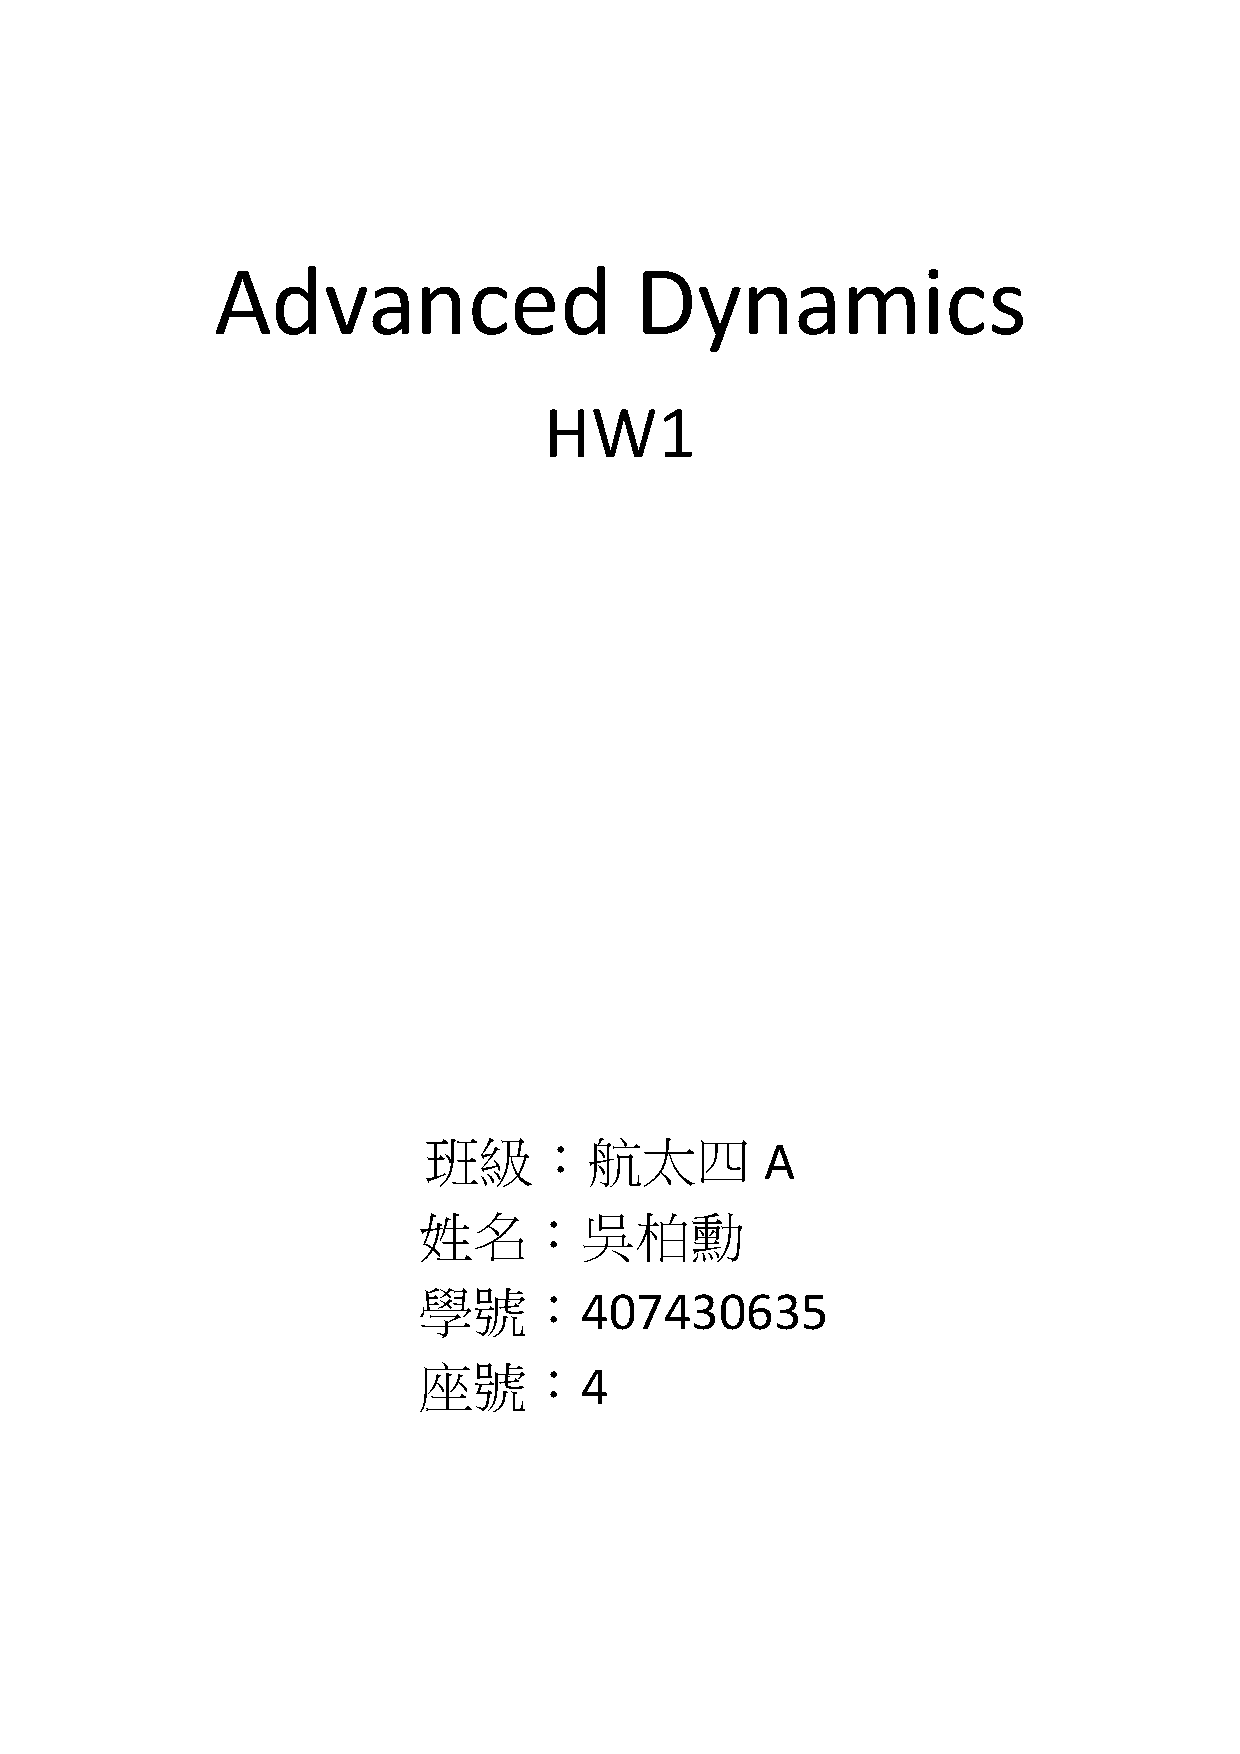
\includepdf[]{../title.pdf}

\section*{Transformation matrices between different frame}

\begin{par}
	From geometry, the unit vector in rotation frame calculated in the fixed frame are
	\begin{equation}
		\label{eq:1}
		\begin{cases}
			\hat{i_1} = \cos{\alpha}\hat{i} + \sin{\alpha}\hat{j} \\
			\hat{j_1} = -\sin{\alpha}\hat{i} + \cos{\alpha}\hat{j} \\
			\hat{k_1} = \hat{k}
		\end{cases}
	\end{equation}
	Rewrite Eq.(\ref{eq:1}) in matrix form
	\begin{equation}
		\label{eq:2}
		\begin{bmatrix}
			\hat{i_1}\\ \hat{j_1}\\ \hat{k_1}
		\end{bmatrix}=
		\begin{bmatrix}
			\cos{\alpha} & \sin{\alpha} & 0 \\
			-\sin{\alpha} & \cos{\alpha} & 0 \\
			0 & 0 & 1
		\end{bmatrix}
		\begin{bmatrix}
			\hat{i}\\ \hat{j}\\ \hat{k}
		\end{bmatrix}\triangleq
		\textbf{T}
		\begin{bmatrix}
			\hat{i}\\ \hat{j}\\ \hat{k}
		\end{bmatrix}
	\end{equation}
	The matrix $T$ is the transfer matrix between fix frame to rotation frame. The transfer matrix between rotation frame to fix frame is the inverse of $T$ ($T^{-1}$).
\end{par}

\dotfill
\subsection*{Matlab program}
\begin{verbatim}
F2R = [ cos(alpha)  sin(alpha)  0       % from fix frame to rotation frame respect to link 1
       -sin(alpha)  cos(alpha)  0
           0           0        1];
R2F = inv(F2R);                         % from rotation frame respect to link 1 to fix frame
\end{verbatim}


\hrulefill
\section*{Position vector of the particle}

\begin{par}
	The position vector of particle 2 in the rotation frame is
	\begin{equation}
		\label{eq:3}
		\textbf{r} = R\cos{\Omega t}\hat{i} + R\sin{\Omega t}\hat{k}
	\end{equation}
	Rewrite Eq.(\ref{eq:3}) in matrix form
	\begin{equation}
		\textbf{r} =
		\begin{bmatrix}
			R\cos{\Omega t}\\ 0\\ R\sin{\Omega t}
		\end{bmatrix}
	\end{equation}
	Then the position vector in the fix frame is
	\begin{equation}
		\textbf{r}_{fix} =
		\begin{bmatrix}
			r_x\\ r_y\\ r_z
		\end{bmatrix} =
		\textbf{T}^{-1}\textbf{r} =
		\begin{bmatrix}
			R\cos{\omega t}\cos{\Omega t}\\ R\sin{\omega t}\cos{\Omega t}\\ R\sin{\Omega t}
		\end{bmatrix}
	\end{equation}
\end{par}

\dotfill
\subsection*{Matlab program}
\begin{verbatim}
r_R = [R*cos(beta) 0 R*sin(beta)]';     % in the rotating frame
r_I = simplify(R2F*r_R);                % in the fix frame
\end{verbatim}


\hrulefill
\section*{Velocity vector of the particle}

\begin{par}
	The velocity vector of the particle 2 in the fix frame is
	\begin{equation}
		\textbf{v}_{fix} = \dot{\textbf{r}}_{fix} =
		\begin{bmatrix}
			-R\omega\sin{\omega t}\cos{\Omega t}-R\Omega\cos{\omega t}\sin{\Omega t}\\
			R\omega\cos{\omega t}\cos{\Omega t}-R\Omega\sin{\omega t}\sin{\Omega t}\\
			R\Omega\cos{\Omega t}
		\end{bmatrix}
	\end{equation}
	Then the velocity vector in the rotating frame  is
	\begin{equation}
		\textbf{v} =
		\begin{bmatrix}
			v_{x1}\\ v_{y1}\\ v_{z1}
		\end{bmatrix} =
		\textbf{T}\textbf{v}_{fix} =
		\begin{bmatrix}
			-R\Omega\sin{\Omega t}\\
			R\omega\cos{\Omega t}\\
			R\Omega\cos{\Omega t}
		\end{bmatrix}
	\end{equation}
\end{par}

\dotfill
\subsection*{Matlab program}
\begin{verbatim}
v_I = diff(r_I,t);                      % in the fix frame
v_R = simplify(F2R*v_I);                % in the rotating frame

fprintf('v_x1 = %s \n',char(v_R(1)))
fprintf('v_y1 = %s \n',char(v_R(2)))
fprintf('v_z1 = %s \n',char(v_R(3)))
fprintf('\n')
\end{verbatim}

\dotfill
\subsection*{Program result}
\begin{verbatim}v_x1 = -OMEGA*R*sin(OMEGA*t)
v_y1 = R*omega*cos(OMEGA*t)
v_z1 = OMEGA*R*cos(OMEGA*t)
\end{verbatim}


\hrulefill
\section*{Acceleration vector of the particle}

\begin{par}
	The acceleration vector of the particle 2 in the fix frame is
	\begin{equation}
		\textbf{a}_{fix} = \dot{\textbf{v}}_{fix} =
		\begin{bmatrix}
			-R\omega^2\cos{\omega t}\cos{\Omega t}+2R\omega\Omega\sin{\omega t}\sin{\Omega t}-R\Omega^2\cos{\omega t}\cos{\Omega t}\\
			-R\omega^2\sin{\omega t}\cos{\Omega t}-2R\omega\Omega\cos{\omega t}\sin{\Omega t}-R\Omega^2\sin{\omega t}\cos{\Omega t}\\
			-R\Omega^2\sin{\Omega t}
		\end{bmatrix}
	\end{equation}
	Then the acceleration vector in the rotating frame  is
	\begin{equation}
		\textbf{a} =
		\begin{bmatrix}
			a_{x1}\\ a_{y1}\\ a_{z1}
		\end{bmatrix} =
		\textbf{T}\textbf{a}_{fix} =
		\begin{bmatrix}
			-R(\Omega^2 + \omega^2)\sin{\Omega t}\\
			-2R\omega\Omega\sin{\Omega t}\\
			-R\Omega^2\sin{\Omega t}
		\end{bmatrix}
	\end{equation}
\end{par}

\dotfill
\subsection*{Matlab program}
\begin{verbatim}
a_I = diff(v_I,t);                      % in the fix frame
a_R = simplify(F2R*a_I);                % in the rotating frame

fprintf('a_x1 = %s \n',char(a_R(1)))
fprintf('a_y1 = %s \n',char(a_R(2)))
fprintf('a_z1 = %s \n',char(a_R(3)))
fprintf('\n')
\end{verbatim}

\dotfill
\subsection*{Program result}
\begin{verbatim}a_x1 = -R*cos(OMEGA*t)*(OMEGA^2 + omega^2)
a_y1 = -2*OMEGA*R*omega*sin(OMEGA*t)
a_z1 = -OMEGA^2*R*sin(OMEGA*t)
\end{verbatim}

\end{document}
